% !TEX program = xelatex
\documentclass[11pt]{article}
\usepackage[margin=1in]{geometry}
\usepackage{nopageno} % no page numbers
\usepackage{setspace}

\usepackage{graphicx}
\graphicspath{ {./graphics/} }
\usepackage[dvipsnames]{xcolor}
\definecolor{CrispBlue}{HTML}{0176AE}

\usepackage{fontspec}
\usepackage{tcolorbox}
\usepackage{etoolbox}
\BeforeBeginEnvironment{verbatim*}{\begin{tcolorbox}[colback=CrispBlue!5!white,colframe=CrispBlue!75!black]}%
\AfterEndEnvironment{verbatim*}{\end{tcolorbox}}%

\usepackage{hyperref}
\hypersetup{
    colorlinks,
    citecolor=black,
    filecolor=black,
    linkcolor=black,
    urlcolor=black
}

\usepackage{subcaption}
\setlength{\parindent}{0pt}
\setlength{\parskip}{1em}

\usepackage{tocloft}
\renewcommand{\cftpartleader}{\cftdotfill{\cftdotsep}}
\renewcommand{\cftsecleader}{\cftdotfill{\cftdotsep}}

\usepackage{fancyhdr}
\pagestyle{fancy}
\fancyhf{}
\lhead{ECE 517: Machine Learning}
\rhead{Assignment 6.2}
\rfoot{Page \thepage}

\usepackage{amsmath,amsfonts,amssymb}
\usepackage{bm}
\usepackage{mathtools}

\renewcommand{\listfigurename}{List of Figures}

\begin{document}
\setmainfont{SF Pro Text}
\setsansfont{SF Pro Text}
\setmonofont{SF Mono}
\renewcommand{\familydefault}{\sfdefault}

\thispagestyle{empty}
\begin{titlepage}
\vspace*{\fill}
\begin{center}
\textsc{\Huge{ECE 517: Machine Learning}}\\[3em]
\textsc{\LARGE Assignment 6.2: Dual Formulation of a Nonlinear\\[0.5em]Classifier With MMSE}\\[6em]
\textsc{\Large David Kirby -- 101652098 -- davidkirby@unm.edu}\\[3em]
\textsc{\Large Fall 2021}
\end{center}
\vfill
\begin{figure}[h]
\begin{subfigure}{0.5\textwidth}

\includegraphics[width=0.25\linewidth]{learning.png}
\end{subfigure}
\begin{subfigure}{0.6\textwidth}\hspace{1em}

\includegraphics[width=0.8\linewidth]{new-soe-logo.png}
\end{subfigure}
\end{figure}
\end{titlepage}
\setcounter{figure}{0}

\hypersetup{
    linkcolor=CrispBlue,
    urlcolor=CrispBlue,
    breaklinks=true
}

\textbf{DUAL FORMULATION OF A NONLINEAR CLASSIFIER WITH MMSE}

Use the functions of the previous assignment to reconstruct the example of lesson 6.1 but using a dual representation and the polynomial kernel \( k (\mathbf{x}_i, \mathbf{x}_j) = (\mathbf{x}_i^\top \mathbf{x}_j + 1)^3\).

\begin{enumerate}
    \item Construct a train dataset and represent them.
    \item Construct a function that computes the kernel matrix \(\mathbf{K}\).
    \item Compute the dual weights \(\alpha _i \) of the MMSE solution.
    \item Write an estimator in dual form as a function of kernel dot products between the training and test data.
    \item Plot the boundary.
    \item Repeat the experiment, but using the Ridge Regression solution, this is
    \begin{equation*}
        \alpha = (\mathbf{K} + \gamma\ \mathbf{I})^{-1}\ y
    \end{equation*}
    where \( \gamma \) is a small number. Show the result for different values of the parameter that are able to produce different solutions. Comment the results.
\end{enumerate}

Provide a document that summarizes the theory and a graph of the result. Comment your results.

\begin{tcolorbox}[colback=CrispBlue!5!white,colframe=CrispBlue!75!black,title=Dual formulation of a non-linear classifier and the polynomial kernel.]\setstretch{1.25}

    To solve the curse of dimensionality, we use the previous equation from Assignment 6.1:
    \begin{equation}
        \mathbf{w} = (\Phi \Phi ^\top)^{-1} \Phi y
    \end{equation}
    
    In primal notation, \(\Phi \Phi ^\top\) is the autocorrelation matrix \(\mathbf{R}\).\\

    Since here we only need a bunch of dot products, we find a dot product that we can easily compute without previously computing the transformation into the Hilbert space. By doing this dot product, we are passing \(\Phi\) that has a number of dimensions into a dual space that has \(N\) dimensions because here we have \(N\) samples. This dual representation keeps the same properties as the primal space.\\

    We will call \(\Phi ^\top \Phi\) the kernel \(\mathbf{K}\), and it is a matrix that contains all the dot products between the data. This kernel trick will allow us to pass from a problem that has a matrix with dimensions equal to the number of dimensions of the space (e.g., 10 or 56) and use a matrix that has dimensions \(N \times N\), where \(N\) is the number of data.\\

    The next step consists of finding a dot product in this higher-dimensional space that can be expressed as a function of the input space only. For our example with the order three Volterra, this dot product is:
    \begin{equation}
        <\phi (\mathbf{x}_n), \phi (\mathbf{x}_m)> = (\mathbf{x}_n^\top \mathbf{x}_m + 1)^3
    \end{equation}

    We can also use Mercer's Theorem, which states that if \(k (\mathbf{x}_n, \mathbf{x}_m)\) exists, gives a real number, and is positive definite, then it is a dot product in the Hilbert space and we can say:
    \begin{equation}
        k (\mathbf{x}_n, \mathbf{x}_m) = <\phi (\mathbf{x}_n), \phi (\mathbf{x}_m)>
    \end{equation}
    
    This dot product in the Hilbert space can be expressed as a function of the vectors in the input space, no longer dependent on \(\Phi\). We can now plug this function into the previous estimator. Thus, using the Representer Theorem and finding a kernel dot product in a space of higher dimension, we solve the curse of dimensionality and then a nonlinear estimator can be constructed by a nonlinear transformation. This allows us to have spaces with a high dimensionality, even infinite, and we don't even notice because we don't go inside the \(\Phi\) dot product.
\end{tcolorbox}
\begin{figure}[h!]
    \centering
    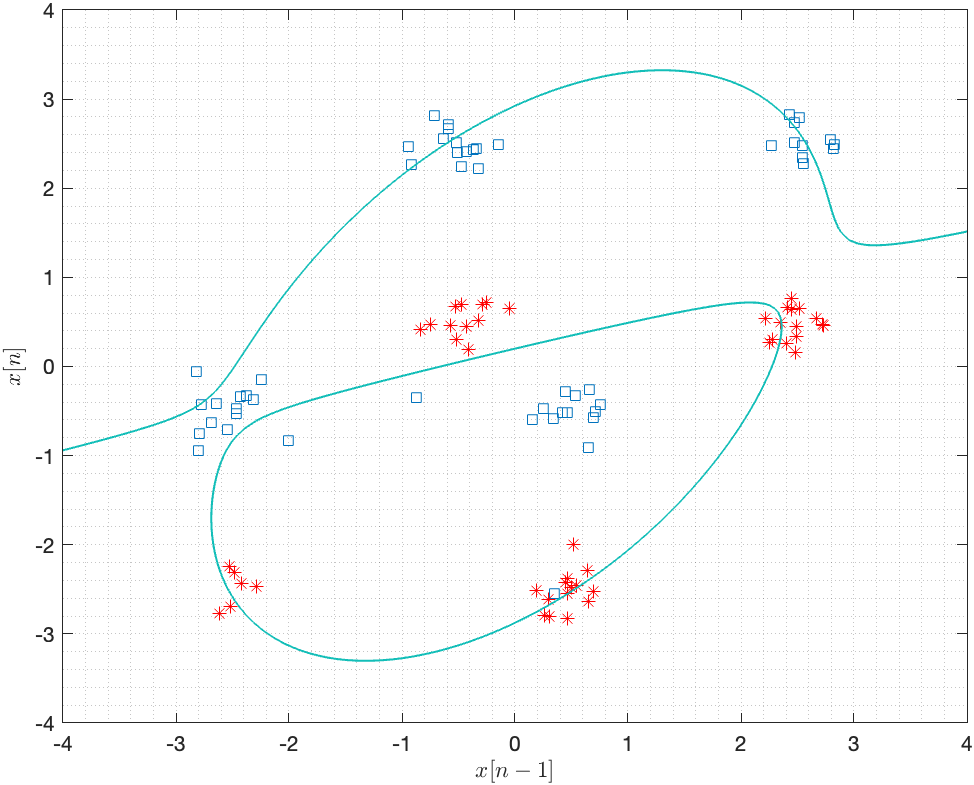
\includegraphics[width=\textwidth]{figure01.png}
    \caption{Dual representation with the polynomial kernel \( k (\mathbf{x}_i, \mathbf{x}_j) = (\mathbf{x}_i^\top \mathbf{x}_j + 1)^3\).}
    \label{fig:figure01}
\end{figure}

\clearpage
\begin{tcolorbox}[colback=CrispBlue!5!white,colframe=CrispBlue!75!black,title=Ridge Regression solution.]\setstretch{1.25}

    Using the properties of kernels, we can expand to Ridge Regression. By comparing figures~\ref{fig:figure01} and~\ref{fig:figure02} we can see that the ridge regression algorithm appears to give a more accurate fit.
    
\end{tcolorbox}
\vspace{1em}
\begin{figure}[h!]
    \centering
    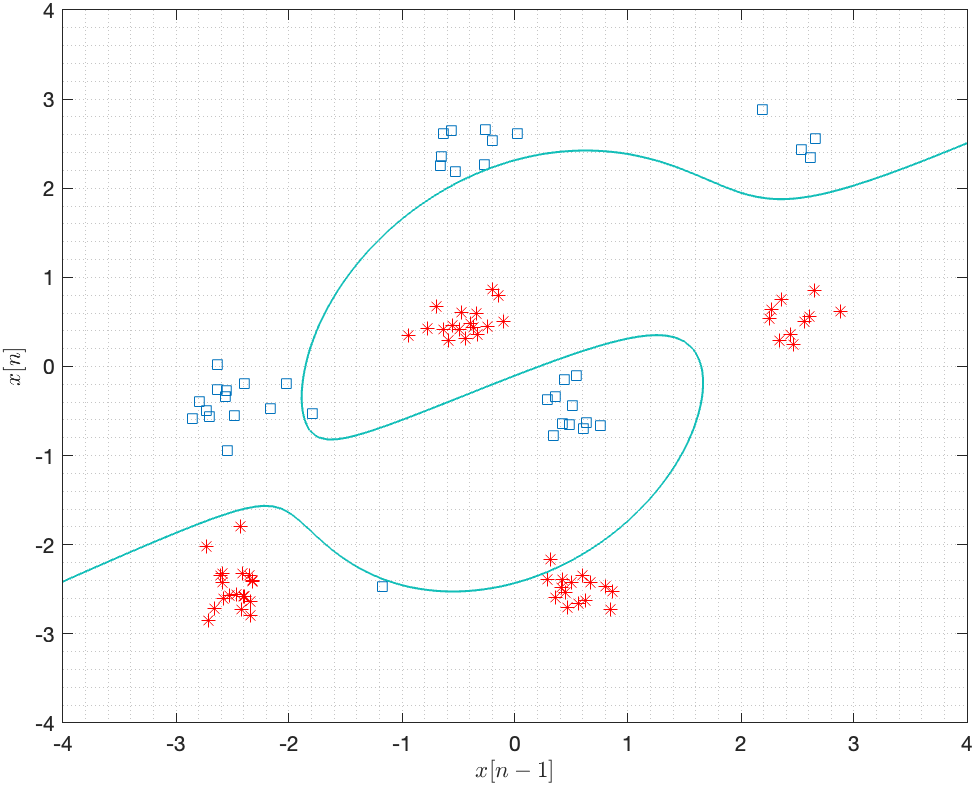
\includegraphics[width=\textwidth]{figure02.png}
    \caption{Ridge regression solution using \(\alpha = (\mathbf{K} + \gamma\ \mathbf{I})^{-1}\ y\).}
    \label{fig:figure02}
\end{figure}

\end{document}